\documentclass[tikz,border=5pt]{standalone}
\usepackage{tikz}
\usetikzlibrary{positioning,fit,backgrounds,calc,arrows.meta}
\usepackage{graphicx}
\usepackage{xcolor}

\definecolor{gitopsblue}{RGB}{51,108,229}
\definecolor{manualgray}{RGB}{102,102,102}
\definecolor{driftred}{RGB}{229,115,115}
\definecolor{okgreen}{RGB}{76,175,80}
\definecolor{metricyellow}{RGB}{251,192,45}
\definecolor{warnorange}{RGB}{255,167,38}

\begin{document}
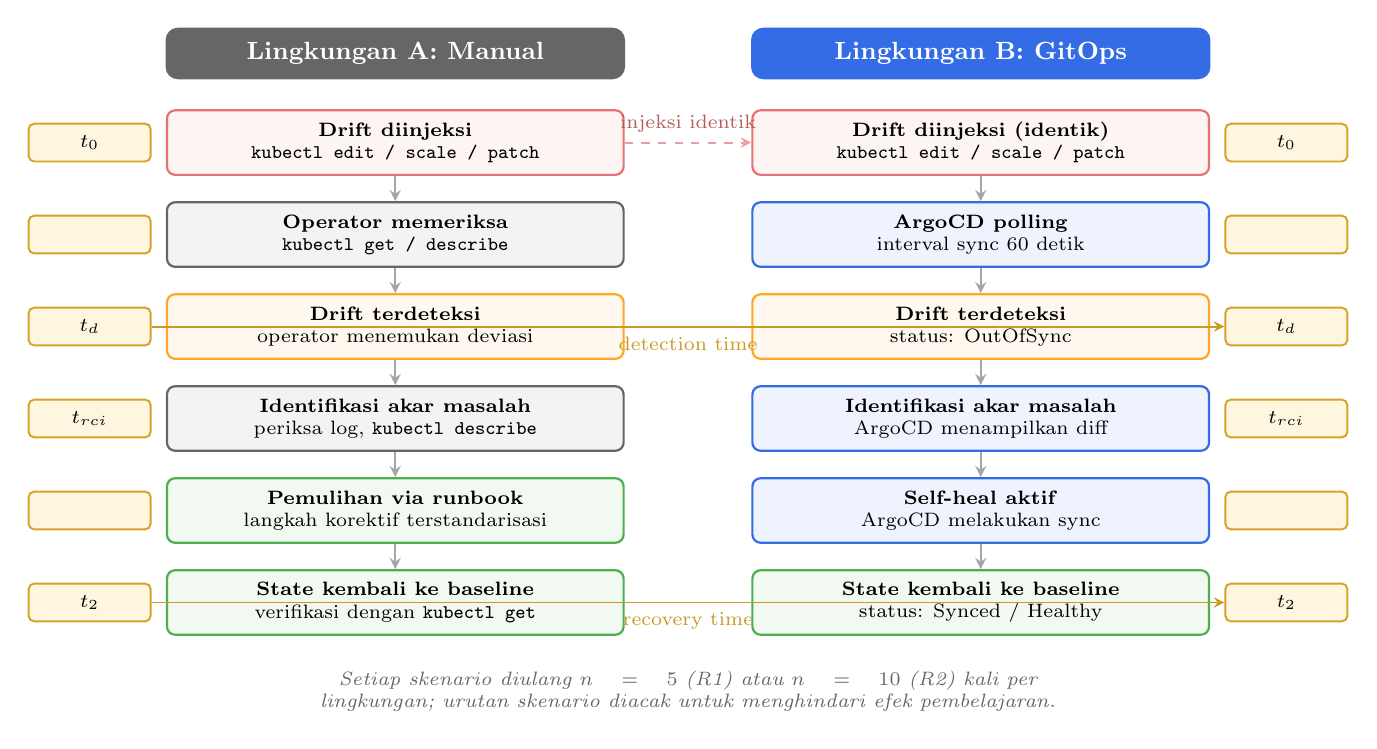
\begin{tikzpicture}[
    node distance=0.32cm and 0.55cm,
    envlabel/.style={rectangle, rounded corners=4pt, draw=#1, fill=#1,
                     text=white, minimum width=5.8cm, minimum height=0.62cm,
                     align=center, font=\small\bfseries, line width=1pt},
    step/.style={rectangle, rounded corners=3pt, draw=#1, fill=#1!8,
                 minimum width=5.8cm, minimum height=0.82cm,
                 align=center, line width=0.8pt, font=\scriptsize},
    timestamp/.style={rectangle, rounded corners=2pt, draw=metricyellow!85!black,
                      fill=metricyellow!15, minimum width=1.55cm,
                      minimum height=0.48cm, align=center,
                      font=\scriptsize\bfseries, line width=0.7pt},
    arrow/.style={->, >=stealth, line width=0.8pt, draw=gray!70},
    midarrow/.style={->, >=stealth, line width=0.7pt, draw=#1},
    note/.style={font=\scriptsize\itshape, text=manualgray}
]

\node[envlabel=manualgray] (aTitle) {Lingkungan A: Manual};

\node[step=driftred, below=0.38cm of aTitle] (a0) {
    \textbf{Drift diinjeksi}\\
    \texttt{kubectl edit / scale / patch}
};
\node[timestamp, left=0.18cm of a0] (ta0) {$t_0$};

\node[step=manualgray, below=of a0] (a1) {
    \textbf{Operator memeriksa}\\
    \texttt{kubectl get / describe}
};
\node[timestamp, left=0.18cm of a1] (ta1) {};

\node[step=warnorange, below=of a1] (a2) {
    \textbf{Drift terdeteksi}\\
    operator menemukan deviasi
};
\node[timestamp, left=0.18cm of a2] (ta2) {$t_d$};

\node[step=manualgray, below=of a2] (a3) {
    \textbf{Identifikasi akar masalah}\\
    periksa log, \texttt{kubectl describe}
};
\node[timestamp, left=0.18cm of a3] (ta3) {$t_{rci}$};

\node[step=okgreen, below=of a3] (a4) {
    \textbf{Pemulihan via runbook}\\
    langkah korektif terstandarisasi
};
\node[timestamp, left=0.18cm of a4] (ta4) {};

\node[step=okgreen, below=of a4] (a5) {
    \textbf{State kembali ke baseline}\\
    verifikasi dengan \texttt{kubectl get}
};
\node[timestamp, left=0.18cm of a5] (ta5) {$t_2$};

\draw[arrow] (a0) -- (a1);
\draw[arrow] (a1) -- (a2);
\draw[arrow] (a2) -- (a3);
\draw[arrow] (a3) -- (a4);
\draw[arrow] (a4) -- (a5);

\node[envlabel=gitopsblue, right=1.6cm of aTitle] (bTitle) {Lingkungan B: GitOps};

\node[step=driftred, below=0.38cm of bTitle] (b0) {
    \textbf{Drift diinjeksi (identik)}\\
    \texttt{kubectl edit / scale / patch}
};
\node[timestamp, right=0.18cm of b0] (tb0) {$t_0$};

\node[step=gitopsblue, below=of b0] (b1) {
    \textbf{ArgoCD polling}\\
    interval sync 60 detik
};
\node[timestamp, right=0.18cm of b1] (tb1) {};

\node[step=warnorange, below=of b1] (b2) {
    \textbf{Drift terdeteksi}\\
    status: OutOfSync
};
\node[timestamp, right=0.18cm of b2] (tb2) {$t_d$};

\node[step=gitopsblue, below=of b2] (b3) {
    \textbf{Identifikasi akar masalah}\\
    ArgoCD menampilkan diff
};
\node[timestamp, right=0.18cm of b3] (tb3) {$t_{rci}$};

\node[step=gitopsblue, below=of b3] (b4) {
    \textbf{Self-heal aktif}\\
    ArgoCD melakukan sync
};
\node[timestamp, right=0.18cm of b4] (tb4) {};

\node[step=okgreen, below=of b4] (b5) {
    \textbf{State kembali ke baseline}\\
    status: Synced / Healthy
};
\node[timestamp, right=0.18cm of b5] (tb5) {$t_2$};

\draw[arrow] (b0) -- (b1);
\draw[arrow] (b1) -- (b2);
\draw[arrow] (b2) -- (b3);
\draw[arrow] (b3) -- (b4);
\draw[arrow] (b4) -- (b5);

\draw[midarrow=driftred!70, dashed] (a0.east) -- (b0.west)
    node[above, font=\scriptsize, text=driftred!80!black, pos=0.5] {injeksi identik};

\draw[midarrow=metricyellow!80!black] (ta2.east) -- (tb2.west)
    node[below, font=\scriptsize, text=metricyellow!80!black, pos=0.5] {detection time};
\draw[midarrow=metricyellow!80!black] (ta5.east) -- (tb5.west)
    node[below, font=\scriptsize, text=metricyellow!80!black, pos=0.5] {recovery time};

\node[note, below=0.32cm of $(a5.south)!0.5!(b5.south)$, text width=13cm, align=center] {
    Setiap skenario diulang $n = 5$ (R1) atau $n = 10$ (R2) kali per lingkungan; urutan skenario diacak untuk menghindari efek pembelajaran.
};

\end{tikzpicture}
\end{document}